Docker is a tool that can package software into containers that run reliably in
any environment \citeWEB{docker-runtime}. One way to package an application is
with a Virtual Machine (VM), where the hardware is simulated and installed with
the required Operating System (OS) and dependencies. It enables the ability to
run multiple applications on the same infrastructure; however, because each VM
runs alongside its OS, they tend to be bulky and slow. A Docker container is
conceptually similar to a VM, but instead of virtualising hardware, containers
only virtualise the OS, which results in faster and more efficient applications
\citeWEB{docker-container-vm}. \Cref{fig:docker_container_vm} demonstrates this
difference.

\begin{figure*}[!htb]
  \centering
  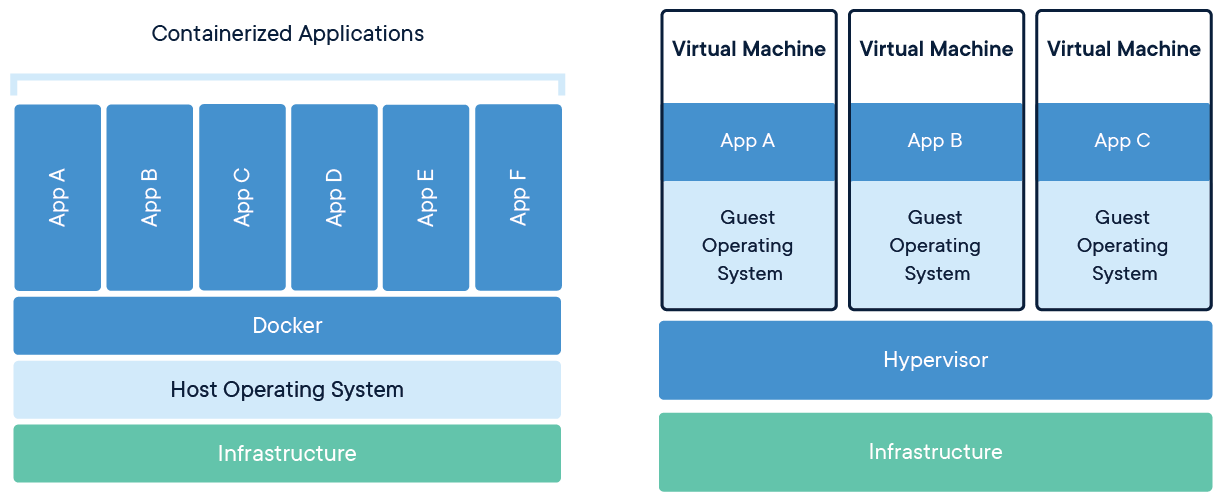
\includegraphics[width=\textwidth]{docker-containerized-and-vm-transparent-bg}
  \caption{Container and Virtual Machines}
  \source{\url{https://www.docker.com/resources/what-container/}}
  \label{fig:docker_container_vm}
\end{figure*}
